\documentclass[12pt, titlepage]{article}

\usepackage{fullpage}
\usepackage[round]{natbib}
\usepackage{multirow}
\usepackage{booktabs}
\usepackage{amssymb}
\usepackage{tabularx}
\usepackage{graphicx}
\usepackage{float}
\usepackage{hyperref}
\hypersetup{
    colorlinks,
    citecolor=blue,
    filecolor=black,
    linkcolor=red,
    urlcolor=blue
}
\usepackage{amsmath}   % For cases/aligned
\usepackage{enumitem}  % For itemize formatting

%% Comments

\usepackage{color}

% \newif\ifcomments\commentstrue %displays comments
\newif\ifcomments\commentsfalse %so that comments do not display

\ifcomments
\newcommand{\authornote}[3]{\textcolor{#1}{[#3 ---#2]}}
\newcommand{\todo}[1]{\textcolor{red}{[TODO: #1]}}
\else
\newcommand{\authornote}[3]{}
\newcommand{\todo}[1]{}
\fi

\newcommand{\wss}[1]{\authornote{blue}{SS}{#1}} 
\newcommand{\plt}[1]{\authornote{magenta}{TPLT}{#1}} %For explanation of the template
\newcommand{\an}[1]{\authornote{cyan}{Author}{#1}}

%% Common Parts

\newcommand{\progname}{Software Engineering} % PUT YOUR PROGRAM NAME HERE
\newcommand{\authname}{\textbf{Team 4, EcoOptimizers} \\
  \\ Nivetha Kuruparan
  \\ Sevhena Walker
  \\ Tanveer Brar
  \\ Mya Hussain
\\ Ayushi Amin} % AUTHOR NAMES

\usepackage{hyperref}
\hypersetup{colorlinks=true, linkcolor=blue, citecolor=blue, filecolor=blue,
urlcolor=blue, unicode=false}
\urlstyle{same}



\newcounter{acnum}
\newcommand{\actheacnum}{AC\theacnum}
\newcommand{\acref}[1]{AC\ref{#1}}

\newcounter{ucnum}
\newcommand{\uctheucnum}{UC\theucnum}
\newcommand{\uref}[1]{UC\ref{#1}}

\newcounter{mnum}
\newcommand{\mthemnum}{M\themnum}
\newcommand{\mref}[1]{M\ref{#1}}

\begin{document}

\title{Module Guide for \progname{}} 
\author{\authname}
\date{\today}

\maketitle

\pagenumbering{roman}

\section{Revision History}

\begin{tabularx}{\textwidth}{p{3cm}p{2cm}X}
\toprule {\bf Date} & {\bf Name} & {\bf Notes}\\
\midrule
January 17th, 2025 & All & Initial draft\\
March 24th, 2025 & All & Added formalization to multiple modules. \\
\bottomrule
\end{tabularx}

\newpage

\section{Reference Material}

This section records information for easy reference.

\subsection{Abbreviations and Acronyms}

\renewcommand{\arraystretch}{1.2}
\begin{tabular}{l l} 
  \toprule		
  \textbf{symbol} & \textbf{description}\\
  \midrule 
  AC & Anticipated Change\\
  DAG & Directed Acyclic Graph \\
  M & Module \\
  MG & Module Guide \\
  OS & Operating System \\
  R & Requirement\\
  SC & Scientific Computing \\
  SRS & Software Requirements Specification\\
  \progname & Explanation of program name\\
  UC & Unlikely Change \\
  VS & Visual Studio\\
  API & Application Programing Interface\\
  IDE & Integrated Development Environment\\
  AST & Abstract Syntax Tree\\
  CSV & Comma-Separated Values\\
  \bottomrule
\end{tabular}\\

\newpage

\tableofcontents

\listoftables

\listoffigures

\newpage

\pagenumbering{arabic}

\section{Introduction}

Decomposing a system into modules is a commonly accepted approach to developing
software.  A module is a work assignment for a programmer or programming
team~\citep{ParnasEtAl1984}.  We advocate a decomposition
based on the principle of information hiding~\citep{Parnas1972a}.  This
principle supports design for change, because the ``secrets'' that each module
hides represent likely future changes.  Design for change is valuable in SC,
where modifications are frequent, especially during initial development as the
solution space is explored.  

Our design follows the rules layed out by \citet{ParnasEtAl1984}, as follows:
\begin{itemize}
\item System details that are likely to change independently should be the
  secrets of separate modules.
\item Each data structure is implemented in only one module.
\item Any other program that requires information stored in a module's data
  structures must obtain it by calling access programs belonging to that module.
\end{itemize}

After completing the first stage of the design, the Software Requirements
Specification (SRS), the Module Guide (MG) is developed~\citep{ParnasEtAl1984}. The MG
specifies the modular structure of the system and is intended to allow both
designers and maintainers to easily identify the parts of the software.  The
potential readers of this document are as follows:

\begin{itemize}
\item New project members: This document can be a guide for a new project member
  to easily understand the overall structure and quickly find the
  relevant modules they are searching for.
\item Maintainers: The hierarchical structure of the module guide improves the
  maintainers' understanding when they need to make changes to the system. It is
  important for a maintainer to update the relevant sections of the document
  after changes have been made.
\item Designers: Once the module guide has been written, it can be used to
  check for consistency, feasibility, and flexibility. Designers can verify the
  system in various ways, such as consistency among modules, feasibility of the
  decomposition, and flexibility of the design.
\end{itemize}

The rest of the document is organized as follows. Section
\ref{SecChange} lists the anticipated and unlikely changes of the software
requirements. Section \ref{SecMH} summarizes the module decomposition that
was constructed according to the likely changes. Section \ref{SecConnection}
specifies the connections between the software requirements and the
modules. Section \ref{SecMD} gives a detailed description of the
modules. Section \ref{SecTM} includes two traceability matrices. One checks
the completeness of the design against the requirements provided in the SRS. The
other shows the relation between anticipated changes and the modules. Section
\ref{SecUse} describes the use relation between modules.

\section{Anticipated and Unlikely Changes} \label{SecChange}

This section lists possible changes to the system. According to the likeliness
of the change, the possible changes are classified into two
categories. Anticipated changes are listed in Section \ref{SecAchange}, and
unlikely changes are listed in Section \ref{SecUchange}.

\subsection{Anticipated Changes} \label{SecAchange}

Anticipated changes are the source of the information that is to be hidden
inside the modules. Ideally, changing one of the anticipated changes will only
require changing the one module that hides the associated decision. The approach
adapted here is called design for
change.

\begin{description}
  \item[\refstepcounter{acnum} \actheacnum \label{acUserInterface}:] The user interface of the plugin. Enhancements may be required to improve usability or accommodate new features. Specific anticipated changes include:
      \begin{itemize}
          \item \textbf{Refactoring Suggestions Display}: Updates to how refactoring suggestions are presented, such as side-by-side views of original and refactored code.
          \item \textbf{Theme Support}: Adding compatibility with various VS Code themes, including light and dark modes.
          \item \textbf{Visual Indicators}: Implementing color-coded indicators to highlight the impact of energy savings for each refactoring suggestion.
          \item \textbf{Interactive Elements}: Introducing interactive components like tooltips or progress indicators to guide users during the refactoring process.
          \item \textbf{Customization Options}: Allowing users to configure UI elements, such as adjusting the sensitivity of code smell detection or selecting preferred refactoring styles.
      \end{itemize}
  
  \item[\refstepcounter{acnum} \actheacnum \label{acVSCodePlugin}:] The VS Code plugin's
    functionality. Future versions may expand to support more complex refactorings
    or additional code smells that users can address with minimal setup. Changes
    may involve adding more customizable user settings.
    
  \item[\refstepcounter{acnum} \actheacnum \label{acRefactorers}:] The refactorers responsible
    for detecting and fixing specific code smells. As more code smells are identified
    and refactoring techniques are developed, new modules may be added or existing
    ones may evolve. For example:
    \begin{itemize}
      \item \textbf{Base Refactorer} \label{acBaseRefactorer}: Updates to the base refactorer module to
      support new refactoring patterns or improved algorithms.
      \item \textbf{Complex List Comprehension} \label{acComplexListComprehension}: Adding or modifying
      the logic for simplifying complex list comprehensions.
      \item \textbf{Long Element Chain} \label{acLongElementChain}: Refining the logic to handle longer
      chains of elements and optimize their readability and performance.
      \item \textbf{Long Lambda Function} \label{acLongLambdaFunction}: Improvements to better handle
      long lambda functions, making them more efficient and readable.
      \item \textbf{Long Message Chain} \label{acLongMessageChain}: Extending the module's ability
      to identify and refactor long message chains.
      \item \textbf{Member Ignoring Method} \label{acMemberIgnoringMethod}: Enhancements to the
      module for detecting methods that ignore members, optimizing the code structure.
      \item \textbf{Repeated Calls} \label{acRepeatedCalls}: Optimizing detection and handling
      of repeated function calls to improve performance.
      \item \textbf{String Concatenation in Loop} \label{acStringConcatenationInLoop}: Adjusting
      the refactorer's logic to improve handling of string concatenation within loops.
      \item \textbf{Long Parameter List} \label{acLongParameterList}: Future extensions to handle
      complex parameter lists in a more structured manner, perhaps allowing for simplifications.
    \end{itemize}
    
  \item[\refstepcounter{acnum} \actheacnum \label{acSmell}:] The core logic
    for identifying specific code smells. As the system evolves, new code smells may be added to the system’s detection capabilities, necessitating changes to this module.
  
  \item[\refstepcounter{acnum} \actheacnum \label{acAnalyzer}:] The analyzers used to
    gather metrics and assess code quality.
  
\end{description}  

\wss{Anticipated changes relate to changes that would be made in requirements,
design or implementation choices.  They are not related to changes that are made
at run-time, like the values of parameters.}

\subsection{Unlikely Changes} \label{SecUchange}

The module design should be as general as possible. However, a general system is
more complex. Sometimes this complexity is not necessary. Fixing some design
decisions at the system architecture stage can simplify the software design. If
these decision should later need to be changed, then many parts of the design
will potentially need to be modified. Hence, it is not intended that these
decisions will be changed.

\begin{description}
  \item[\refstepcounter{ucnum} \uctheucnum \label{ucPlatform}:] Transitioning from VS Code to another IDE. The plugin is tightly integrated with VS Code's API, making such a change complex.
  \item[\refstepcounter{ucnum} \uctheucnum \label{ucCoreLogic}:] Fundamental changes to the core logic of code smell detection. The current architecture is designed around widely accepted principles of software quality.
  \item[\refstepcounter{ucnum} \uctheucnum \label{ucPluginType}:] Changing from a plugin-based architecture to a standalone application. This would require rethinking the entire deployment and user interaction model.
\end{description}

\section{Module Hierarchy} \label{SecMH}

This section provides an overview of the module design. Modules are summarized
in a hierarchy decomposed by secrets in Table \ref{TblMH}. The modules listed
below, which are leaves in the hierarchy tree, are the modules that will
actually be implemented.

\begin{description}
  \item [\refstepcounter{mnum} \mthemnum \label{mSmell}:] Smell Module
  \item [\refstepcounter{mnum} \mthemnum \label{mBR}:] BaseRefactorer Module
  \item [\refstepcounter{mnum} \mthemnum \label{mMIMR}:] MakeStaticRefactorer Module
  \item [\refstepcounter{mnum} \mthemnum \label{mSCLR}:] UseListAccumulationRefactorer Module
  \item [\refstepcounter{mnum} \mthemnum \label{mUGENR}:] UseAGeneratorRefactorer Module
  \item [\refstepcounter{mnum} \mthemnum \label{mCRC}:] CacheRepeatedCallsRefactorer Module
  \item [\refstepcounter{mnum} \mthemnum \label{mLEC}:] LongElementChainRefactorer Module
  \item [\refstepcounter{mnum} \mthemnum \label{mLPL}:] LongParameterListRefactorer Module
  \item [\refstepcounter{mnum} \mthemnum \label{mLMC}:] LongMessageChainRefactorer Module
  \item [\refstepcounter{mnum} \mthemnum \label{mLLF}:] LongLambdaFunctionRefactorer Module
  \item [\refstepcounter{mnum} \mthemnum \label{mExe}:] Plugin Initiator Module
  \item [\refstepcounter{mnum} \mthemnum \label{mBac}:] Backend Communicator Module
  \item [\refstepcounter{mnum} \mthemnum \label{mDet}:] Smell Detector Module
  \item [\refstepcounter{mnum} \mthemnum \label{mHig}:] File Highlighter Module
  \item [\refstepcounter{mnum} \mthemnum \label{mHov}:] Hover Manager Module
  \item [\refstepcounter{mnum} \mthemnum \label{mMeasure}:] Measurements Module
  \item [\refstepcounter{mnum} \mthemnum \label{mPyA}:] Pylint Analyzer Module
  \item [\refstepcounter{mnum} \mthemnum \label{mRef}:] Smell Refactorer  Module
  \item [\refstepcounter{mnum} \mthemnum \label{mMan}:] Refactor Manager Module
  \item [\refstepcounter{mnum} \mthemnum \label{mCac}:] Cache Manager Module
  \item [\refstepcounter{mnum} \mthemnum \label{mFil}:] Filter Manager Module
  \item [\refstepcounter{mnum} \mthemnum \label{mEne}:] Energy Metrics Module
  \item [\refstepcounter{mnum} \mthemnum \label{mVie}:] View Provider Module
  \item [\refstepcounter{mnum} \mthemnum \label{mEve}:] Event Manager Module
\end{description}


\begin{table}[h!]
  \centering
  \begin{tabular}{p{0.3\textwidth} p{0.6\textwidth}}
  \toprule
  \textbf{Level 1} & \textbf{Level 2}\\
  \midrule
  
  {Hardware-Hiding Module} & None \\
  \midrule
  
  \multirow{7}{0.3\textwidth}{Behaviour-Hiding Module} & Smell Module\\
  & BaseRefactorer Module\\
  & MakeStaticRefactorer Module\\
  & UseListAccumulationRefactorer Module\\
  & UseAGeneratorRefactorer Module\\
  & CacheRepeatedCallsRefactorer Module\\
  & LongElementChainRefactorer Module\\
  & LongParameterListRefactorer Module\\
  & LongMessageChainRefactorer Module\\
  & LongLambdaFunctionRefactorer Module\\ 
  & PluginInitiator Module\\
  & BackendCommunicator Module\\ 
  & SmellDetector Module\\
  & FileHighlighter Module\\
  & HoverManager Module\\
  & CacheManager Module\\
  & FilterManager Module\\
  \midrule


  \multirow{3}{0.3\textwidth}{Software Decision Module} & Measurements Module\\
& PylintAnalyzer Module\\
& SmellRefactorer Module\\
& RefactorManager Module\\
& EnergyMetrics Module\\
& ViewProvider Module\\
& EventManager Module\\
\bottomrule

\end{tabular}
\caption{Module Hierarchy}
\label{TblMH}
\end{table}

\section{Connection Between Requirements and Design} \label{SecConnection}

The design of the system is intended to satisfy the requirements developed in
the SRS. In this stage, the system is decomposed into modules. The connection
between requirements and modules is listed in Table~\ref{TblRT}.

\wss{The intention of this section is to document decisions that are made
  ``between'' the requirements and the design.  To satisfy some requirements,
  design decisions need to be made.  Rather than make these decisions implicit,
  they are explicitly recorded here.  For instance, if a program has security
  requirements, a specific design decision may be made to satisfy those
  requirements with a password.}

\section{Module Decomposition} \label{SecMD}

Modules are decomposed according to the principle of ``information hiding''
proposed by \citet{ParnasEtAl1984}. The \emph{Secrets} field in a module
decomposition is a brief statement of the design decision hidden by the
module. The \emph{Services} field specifies \emph{what} the module will do
without documenting \emph{how} to do it. For each module, a suggestion for the
implementing software is given under the \emph{Implemented By} title. If the
entry is \emph{OS}, this means that the module is provided by the operating
system or by standard programming language libraries.  \emph{\progname{}} means the
module will be implemented by the \progname{} software.

Only the leaf modules in the hierarchy have to be implemented. If a dash
(\emph{--}) is shown, this means that the module is not a leaf and will not have
to be implemented.

\subsection{Hardware Hiding Modules}

This system has no hardware components.

\subsection{Behaviour-Hiding Module}

\subsubsection{Smell Module (\mref{mSmell})}

\begin{description}
\item[Secrets:] Data structure of a code smell.
\item[Services:] Provides an interface for other modules to access information of a smell object.
\item[Implemented By:] EcoOptimizer
\item[Type of Module:] Abstract Data Type
\end{description}

\subsubsection{Base Refactorer Module (\mref{mBR})}

% [Record, Library, Abstract Object, or Abstract Data Type]

\begin{description}
    \item[Secrets:] None
    \item[Services:] Offers an interface for other refactoring modules to implement.
    \item[Implemented By:] EcoOptimizer
\end{description}

\subsubsection{MakeStaticRefactorer Module (\mref{mMIMR})}

% [Record, Library, Abstract Object, or Abstract Data Type]
\begin{description}
\item[Secrets:] How to parse a given code file to its AST representation, how to traverse the AST tree, how to modify specific nodes in the AST tree, how to convert the modified AST tree back to source code and write it to an output file.
\item[Services:] Refactors the \textit{\textbf{Member Ignoring Method (MIM)}} smell in a provided code file to improve energy efficiency.
\item[Implemented By:] EcoOptimizer
\item[Type of Module:] Abstract Object: A transformation component that modifies Python source code to optimize method calls.
\end{description}

\textbf{Formalization of MakeStaticRefactorer}

\begin{enumerate}
  \item \textbf{Definitions}
  \begin{itemize}
      \item \textit{Source Code}: A Python program \( D \) consisting of a set of statements \( S = \{ s_1, s_2, \dots, s_n \} \).
      \item \textit{Member Ignoring Method (MIM)}: A function \( f \) defined inside a class \( C \) that does not use instance attributes or methods.
      \item \textit{Static Method Transformation}: A function \( T \) that converts an instance method \( f \) into a static method \( f' \), where:
      \[
      T(f) = f' \text{ such that } \forall x \in C, f(x) = f'
      \]
      \item \textit{Refactored Code}: The transformed version of \( D \), denoted as \( D' \), where all applicable \( f \) are replaced by \( f' \).
  \end{itemize}

  \item \textbf{Transformation Process}
  \begin{itemize}
      \item Parse \( D \) into an AST representation.
      \item Identify functions \( f \) where:
      \begin{itemize}
          \item \( f \in C \) (i.e., \( f \) is a method within a class).
          \item \( f \) does not reference any instance variables.
      \end{itemize}
      \item Modify \( f \) by:
      \begin{itemize}
          \item Adding a `@staticmethod` decorator.
          \item Removing the `self` parameter from its signature.
      \end{itemize}
      \item Update all relevant method calls in \( D \) to reflect the static method transformation.
  \end{itemize}

  \item \textbf{Validation and Constraints}
  \begin{itemize}
      \item Ensure correctness by preserving method functionality.
      \item Verify that method calls in \( D \) remain semantically valid after transformation.
      \item Maintain compatibility with subclasses and inherited methods.
  \end{itemize}
\end{enumerate}

\subsubsection{UseListAccumulationRefactorer Module (\mref{mSCLR})}

% [Record, Library, Abstract Object, or Abstract Data Type]

\begin{description}
\item[Secrets:] How to parse a given code file into its AST representation, how to traverse the AST tree, how to find the initializing variable of the string concatenation, how to find the scope of the concatenation, how to modify the given code file in plain text and write it back to an output file.
\item[Services:] Refactors the \textbf{\textit{String Concatenation Inside Loop (SCL)}} smell in a provided code file to improve energy efficiency.
\item[Implemented By:] EcoOptimizer
\end{description}

\subsubsection{UseAGeneratorRefactorer Module (\mref{mUGENR})}
\begin{description}
    \item[Secrets:] How to parse a given code file to its AST representation, how to traverse the AST tree, how to modify specific nodes in the AST tree, how to convert the modified AST tree back to source code and write it to an output file.
    \item[Services:] Refactors the \textbf{\textit{List Comprehension Instead of a Generator}} smell in a provided code file to improve energy efficiency.
    \item[Implemented By:] EcoOptimizer
\end{description}

\subsubsection{CacheRepeatedCallsRefactorer Module (\mref{mCRC})}
\begin{description}
    \item[Secrets:] How to parse a given code file to its AST representation, how to traverse the AST tree, how to modify specific nodes in the AST tree, how to convert the modified AST tree back to source code and write it to an output file.
    \item[Services:] Refactors the \textbf{\textit{Repeated Function Calls}} smell in a provided code file to improve energy efficiency and performance.
    \item[Implemented By:] EcoOptimizer
\end{description}

\subsubsection{Long Element Chain Module (\mref{mLEC})}

\begin{description}
    \item[Secrets:] How to parse a given code file to its AST representation, traverse the 
    AST tree to identify dictionary assignments, analyze the structure of nested dictionaries,
     and flatten them. Additionally, it identifies all access calls associated with these dictionaries
      in the source code and determines how to update them to reflect the new flattened structure.
    \item[Services:] Detects nested dictionaries in the source code using AST parsing, simplifies their 
    structure by flattening them, and updates all associated access calls throughout the file. This improves 
    code readability, reduces complexity, and ensures correctness while maintaining the program's intended behavior.
    \item[Implemented By:] EcoOptimizer
    \item[Type of Module:] Library: provides functionality for refactoring nested dictionary structures in Python code.
\end{description}

\textbf{Long Element Chain Formalization}
\begin{enumerate}
  \item \textbf{Definitions}
  \begin{itemize}
      \item \textit{Nested Dictionary}: Dictionary \( D = \{k_1: \{k_2: \dots \{k_n: v\}\}\} \)
      \item \textit{Flattened Dictionary}: \( D' = \{k_1\_k_2\_\dots\_k_n: v\} \)
      \item \textit{Access Path}: Sequence \( P = [k_1, k_2, \dots, k_n] \)
      \item \textit{Composite Key}: String \( c_k = \text{join}(P, "\_") \)
      \item \textit{Indentation}: Leading whitespace \( W \) from original code
  \end{itemize}

  \item \textbf{Refactoring Function}
  \begin{itemize}
      \item Dictionary Flattening:
      \[
      \begin{aligned}
          &\forall\ \text{nested path } P \in D,\ \exists\ c_k \in D' \\
          &D'[c_k] = D[P_1][P_2]\dots[P_n] \quad \text{(preserve } W\text{)}
      \end{aligned}
      \]
      
      \item Access Path Update:
      \[
      \begin{aligned}
          &\text{Original Access: } &D[P_1][P_2]\dots[P_n] \\
          &\text{Refactored Access: } &D'[c_k] \quad \text{where } c_k = \text{join}(P, "\_") 
      \end{aligned}
      \]
  \end{itemize}
\end{enumerate}

\subsubsection{Long Parameter List Module (\mref{mLPL})}

% [Record, Library, Abstract Object, or Abstract Data Type]

\begin{description}
    \item[Secrets:] How to parse a given code file to its AST representation, traverse the AST tree to identify functions or methods with long parameter lists, and encapsulate related parameters into objects or structures. Additionally, it identifies all function or method calls associated with these functions and updates their arguments to align with the refactored signature.
    \item[Services:] Detects long parameter lists in functions or methods using AST parsing, simplifies their structure by grouping related parameters into objects or structures, and updates all associated function or method calls throughout the file. This improves code readability, reduces complexity, and ensures correctness while maintaining the program’s intended behavior.
    \item[Implemented By:] EcoOptimizer
\end{description}

\subsubsection{Long Message Chain Refactorer (\mref{mLMC})}


\begin{description}
    \item[Secrets:] Understanding the syntax and structure of Python code to identify/classify long message chains, including both f-strings and non-f-string chains. This involves parsing the target file, extracting method calls from identified long chains, and systematically breaking them into separate statements while preserving the original functionality and indentation. Additionally, it ensures unmatched brackets are corrected during refactoring.
    
    \item[Services:] Detects long message chains in Python source code and refactors them by splitting the chain into intermediate variables and a final result. This improves code readability and maintainability while retaining the original program behavior. 

    \item[Implemented By:] EcoOptimizer
    \item[Type of Module:] Library: a reusable component that provides functionality for refactoring long message chains in Python code.
   
\end{description}

\textbf{Long Message Chain Formalization}
\begin{enumerate}
  \item \textbf{Definitions}
  \begin{itemize}
      \item \textit{Input Line}: String \( L \) (e.g., \texttt{obj.a().b().c()})
      \item \textit{Method Chain}: Sequence \( M = [m_1, m_2, \dots, m_n] \), where \( m_i \) is a method call
      \item \textit{Intermediate Variables}: Generated variables \( V = [v_0, v_1, \dots, v_{n-1}] \)
      \item \textit{Indentation}: Leading whitespace \( W \) from \( L \)
  \end{itemize}

  \item \textbf{Refactoring Function}
  \begin{itemize}
      \item For f-strings:
      \[
      \begin{aligned}
          &v_0 = f_{\text{str}} \quad \text{(preserve } W\text{)} \\
          &v_1 = v_0.m_1 \quad \text{(preserve } W\text{)} \\
          &\;\;\vdots \\
          &\text{result} = v_{n-1}.m_n \quad \text{(preserve } W\text{)}
      \end{aligned}
      \]
      \item For regular chains:
      \[
      \begin{aligned}
          &v_0 = m_1 \quad \text{(preserve } W\text{)} \\
          &v_1 = v_0.m_2 \quad \text{(preserve } W\text{)} \\
          &\;\;\vdots \\
          &\text{result} = v_{n-1}.m_n \quad \text{(preserve } W\text{)}
      \end{aligned}
      \]
  \end{itemize}
\end{enumerate}


\subsubsection{Long Lambda Function Refactorer (\mref{mLLF})}


\begin{description} 
  \item[Secrets:] Understanding the syntax and structure of Python code to identify long lambda functions. This includes parsing the target file to locate lambda expressions, extracting their arguments and bodies, and converting them into standard Python function definitions. The module ensures proper handling of nested structures (e.g., parentheses, brackets, and braces) within the lambda body, and truncates overly complex expressions at the first top-level comma for readability.

  \item[Services:] Detects components of long lambda functions in Python source code and refactors them by converting the lambda expression into a standalone function with a unique name. This improves code readability, debugging, and maintainability. The module inserts the newly defined function in the appropriate scope, updates the original lambda usage with a function call, and validates the refactored code by maintaining its functionality and measuring energy efficiency improvements.

  \item[Implemented By:] EcoOptimizer
  
  \item[Type of Module:] Library: a reusable component that provides functionality for refactoring long lambda functions in Python code.
\end{description}

\textbf{Long Lambda Function Formalization}
\begin{enumerate}
  \item \textbf{Definitions}
  \begin{itemize}
      \item \textit{Lambda Expression}: String \( L = \text{``lambda'' }A\text{``:'' }B \) where:
      \begin{itemize}
          \item \( A = [a_1, \dots, a_n] \) : Formal parameters
          \item \( B \) : Body expression
      \end{itemize}
      
      \item \textit{Truncated Body}: \( B' = \begin{cases} 
          B[0:i] & \text{if top-level comma at } i \\
          B & \text{otherwise}
      \end{cases} \)
      
      \item \textit{Function Name}: \( F = \text{``converted\_lambda\_''} + \text{line\_num} \)
      
      \item \textit{Indentation}:
      \begin{itemize}
          \item \( W \) : Original line's whitespace
          \item \( W_c \) : Parent block indentation
          \item \( D = 4 \) : Indentation delta (spaces)
      \end{itemize}
  \end{itemize}

  \item \textbf{Transformation Rules}
  \begin{itemize}
      \item \textbf{Function Generation}:
      \[
      \begin{aligned}
          &\textsc{Definition}: & W_c\text{``def ''}F(A)\text{``:''} \\
          &\textsc{Body}: & (W_c + D)\text{``result = ''}B' \\
          &\textsc{Return}: & (W_c + D)\text{``return result''}
      \end{aligned}
      \]
      
      \item \textbf{Lambda Replacement}:
      \[
      W\text{``lambda ''}A\text{``: ''}B \quad \Rightarrow \quad W F
      \]
  \end{itemize}

  \item \textbf{Example}
  \begin{itemize}
      \item \textit{Before}:
      \begin{verbatim}
      # Original lambda (line 42)
      result = map(lambda x: x**2, data)
      \end{verbatim}
      
      \item \textit{After}:
      \begin{verbatim}
def converted_lambda_42(x):    # W_c = ""
    result = x**2             # W_c + D (D=4)
    return result

      result = map(converted_lambda_42, data)
      \end{verbatim}
  \end{itemize}
\end{enumerate}

\textit{Key Relationships}:
\begin{itemize}
    \item \( F \) uniqueness via \text{line\_num}
    \item \( D = 4 \) ensures PEP8 compliance
    \item \( W \) preservation maintains code structure
\end{itemize}

\textit{Key Relationships}:
\begin{itemize}
    \item \( F \) preserves lexical scope via \( W_c \) alignment
    \item \( B' \) ensures syntactic validity through comma truncation
    \item \( \Delta = 4 \) enforces PEP8 indentation rules
    \item \( W \) retention maintains original code structure
\end{itemize}

\subsubsection{Plugin Initiator Module (\mref{mExe})}

% [Record, Library, Abstract Object, or Abstract Data Type]

\begin{description}
    \item[Secrets:] How to initialize the plugin, set up the environment for interaction, and handle configurations for plugin commands.
    \item[Services:] Initializes and manages the plugin's setup including command registration, enabling its functionality without exposing the underlying initialization logic.
    \item[Implemented By:] EcoOptimizer
\end{description}

\subsubsection{Backend Communicator (\mref{mBac})}

% [Record, Library, Abstract Object, or Abstract Data Type]

\begin{description}
    \item[Secrets:] How to establish communication between the plugin and Source Code Optimizer, handle requests, and process responses.
    \item[Services:] Provides an interface for sending requests to and receiving responses from Source Code Optimizer. Abstracts the communication details from modules within the plugin. Managers server status checks and handles backend communication errors.
    \item[Implemented By:] EcoOptimizer
\end{description}

\subsubsection{Smell Detector (\mref{mDet})}

% [Record, Library, Abstract Object, or Abstract Data Type]

\begin{description}
    \item[Secrets:] How to analyze Python code in active VS Code editor by accessing Source Code Optimizer endpoint.
    \item[Services:] Detects code smells in Python scripts using Source Code Optimizer and provides structured data for further processing based on received output.
    \item[Implemented By:] EcoOptimizer
    \item[Type of Module:] Abstract Object: A component responsible for code smell detection and classification.
\end{description}

\textbf{Smell Detection Formalization}
\begin{enumerate}
  \item \textbf{Definitions}
  \begin{itemize}
      \item \textit{Source Code}: A document \( D \) containing a sequence of statements \( S = \{ s_1, s_2, \dots, s_n \} \).
      \item \textit{Code Smell}: A property \( C_k \) that signifies a potential issue in \( D \), where:
      \[
      C_k = \{ c_1, c_2, \dots, c_m \}
      \]
      represents a set of detectable code smells.
      \item \textit{Detection Function}: A mapping \( F: D \to C_k \), which evaluates \( D \) and returns a set of identified smells.
      \item \textit{Smell Report}: A structured output \( R \) summarizing detected smells and their locations in \( D \).
  \end{itemize}

  \item \textbf{Detection Process}
  \begin{itemize}
      \item Extract syntactic and semantic features from \( D \).
      \item Apply detection rules to identify instances of \( C_k \).
      \item Generate a structured smell report \( R \) containing:
      \begin{itemize}
          \item Smell type \( c_i \)
          \item Line number(s) \( L = \{ l_1, l_2, \dots, l_p \} \)
          \item Severity level \( \sigma \) based on predefined metrics
      \end{itemize}
  \end{itemize}

  \item \textbf{Classification and Output}
  \begin{itemize}
      \item Structure \( R \) for further analysis by the refactoring module.
      \item Ensure results are accessible to downstream processing components.
  \end{itemize}

  \item \textbf{Validation and Adaptation}
  \begin{itemize}
      \item Maintain a feedback loop to refine detection accuracy.
      \item Adapt detection parameters based on observed refactoring effectiveness.
  \end{itemize}
\end{enumerate}

\subsubsection{File Highlighter Module (\mref{mHig})}

% [Record, Library, Abstract Object, or Abstract Data Type]

\begin{description}
    \item[Secrets:] How to identify code regions requiring attention and how to highlight those regions in the file.
    \item[Services:] Highlights areas in files that contain code smells and can be refactored, assisting developers in identifying problem areas quickly.
    \item[Implemented By:] EcoOptimizer
\end{description}


\subsubsection{Hover Manager Module (\mref{mHov})}

\begin{description}
    \item[Secrets:] Understanding how to detect hover events over source code, retrieve relevant contextual information dynamically, and generate structured hover content. This includes identifying code smells at a given position, constructing a `MarkdownString` representation, and embedding interactive refactoring commands.

    \item[Services:] Manages hover interactions within the VSCode extension. When a user hovers over a detected code smell, it dynamically provides a `MarkdownString` containing information about the smell and options to refactor it. The module supports both single-instance and type-wide refactoring actions.

    \item[Implemented By:] EcoOptimizer
    \item[Type of Module:] Library: a reusable component responsible for handling hover events and providing interactive refactoring commands within the extension.
\end{description}

\textbf{Hover Interaction Formalization}
\begin{enumerate}
  \item \textbf{Definitions}
  \begin{itemize}
      \item \textit{Interaction Space}: A document \( D \) consisting of discrete positions \( P = \{ p_1, p_2, \dots, p_n \} \) where detected smells can be associated.
      \item \textit{Smell Data}: A set \( S = \{ s_1, s_2, \dots, s_m \} \), where each \( s_i \) is a detected smell with:
        \begin{itemize}
            \item \( s_i.\text{location} \) — position range where the smell occurs
            \item \( s_i.\text{description} \) — information about the smell
        \end{itemize}
      \item \textit{Response Function}: A mapping \( H: P \to S \) that associates positions in \( D \) with detected smells.
  \end{itemize}

  \item \textbf{Interaction Model}
  \[
  H(p) =
  \begin{cases} 
      s_i, & \text{if } p \text{ corresponds to a detected smell} \\
      \varnothing, & \text{otherwise}
  \end{cases}
  \]

  \item \textbf{Contextual Response Construction}
  \begin{itemize}
      \item Given \( p \in P \), retrieve \( s_i \in S \).
      \item Construct a structured response containing \( s_i.\text{description} \) and \( s_i.\text{transformationOptions} \).
      \item Present the response in an interactive format that allows further refinement or transformation.
  \end{itemize}
\end{enumerate}

\subsubsection{Cache Manager Module (\mref{mCac})}

\begin{description}
    \item[Secrets:] How to persist and retrieve smell detection results, manage cache invalidation, handle cache state transitions and synchronize cache with file system changes. 
    \item[Services:] Provides persistent storage for smell detection results and the ability to retrieve cached smell data, invalidate cache entries for specific files, clear entire cache.  Coordinates cache updates with file system events. 
    \item[Implemented By:] EcoOptimizer
\end{description}

\subsubsection{Filter Manager Module (\mref{mFil})}

\begin{description}
    \item[Secrets:] How to handle and respond to filter criteria across sessions. How to handle filter combinations concurrently with UI synchronization.
    \item[Services:] Provides functionality to set and get filter criteria for different smell types and apply filters to smell data. This module can clear all active filters, save filter state to persistent storage, restore filter state from storage and validate filter criteria.
    \item[Implemented By:] EcoOptimizer
\end{description}

\subsection{Software Decision Module}

\subsubsection{Measurements Module (\mref{mMeasure})}

\begin{description}
\item[Secrets:] How to measure energy consumption and carbon emissions of a given Python program using the CodeCarbon library, including managing temporary directories for storing output, executing the program, and processing the emissions data from a CSV file.
\item[Services:] Provides functionality for measuring the energy consumption and carbon emissions of a provided code file. This module handles execution, tracking, and data extraction, ensuring that the emissions data is available for further analysis.
\item[Implemented By:] CodeCarbonEnergyMeter
\end{description}

\subsubsection{Pylint Analyzer Module (\mref{mPyA})}

\begin{description}
\item[Secrets:] The internal design and execution of static code analysis using Pylint and AST parsing, including custom detection and structuring of smells. These details are hidden from external modules.
\item[Services:] The module provides the following services:
  \begin{itemize}
    \item Executes Pylint analysis on Python source code files.
    \item Performs AST-based custom checks for specific code smells.
    \item Filters and structures the analysis results into a standardized format for further processing.
  \end{itemize}
\item[Implemented By:] \texttt{EcoOptimizer}
\end{description}


\subsubsection{Smell Refactorer Module (\mref{mRef})}

% [Record, Library, Abstract Object, or Abstract Data Type]

\begin{description}
    \item[Secrets:] How to utilize Source Code Optimizer endpoint for refactoring specific code smells, and how to sanitize received output.
    \item[Services:] Refactors code smells in Python scripts using Source Code Optimizer and determines if received output is valid format.
    \item[Implemented By:] EcoOptimizer
\end{description}


\subsubsection{Refactor Manager Module (\mref{mMan})}

\begin{description}
    \item[Secrets:] How to coordinate the sequence of refactorings, apply transformations to source code while maintaining correctness, validate the impact of each step, and enable reversion when necessary. Ensures that refactoring operations preserve program behavior.

    \item[Services:] Manages the execution of refactorings, determines whether modifications should be committed to the source file, and allows users to revert changes if needed.

    \item[Implemented By:] EcoOptimizer
    \item[Type of Module:] Abstract Object: A conceptual entity that organizes and controls the refactoring process.
\end{description}

\textbf{Refactoring Execution Formalization}
\begin{enumerate}
  \item \textbf{Definitions}
  \begin{itemize}
      \item \textit{Source Code}: A document \( D \) consisting of a sequence of statements \( S = \{ s_1, s_2, \dots, s_n \} \).
      \item \textit{Code Smell}: An identified issue \( \sigma \) in \( D \) that may impact maintainability, readability, or performance.
      \item \textit{Refactoring Rule}: A transformation function \( R: D \to D' \) that modifies \( S \) while improving energy consumption.
      \item \textit{Refactoring Sequence}: An ordered set of transformations \( \mathcal{R} = [R_1, R_2, \dots, R_m] \) applied sequentially to \( D \).
  \end{itemize}

  \item \textbf{Refactoring Process}
  \begin{itemize}
      \item Given a detected smell \( \sigma \), identify the corresponding transformation \( R_{\sigma} \).
      \item Apply \( R_{\sigma} \) to \( D \), producing \( D' \).
      \item Track all modifications to ensure consistency and correctness.
  \end{itemize}

  \item \textbf{Modification Tracking}
  \begin{itemize}
      \item Maintain a count of applied transformations per smell type:  
        \[
        C_{\sigma} = C_{\sigma} + 1
        \]
      \item Store modified versions of \( D \) to enable rollback.
      \item Generate output files when refactoring is applied.
  \end{itemize}

  \item \textbf{Validation and Reversion}
  \begin{itemize}
      \item After applying \( R_{\sigma} \), verify correctness:  
        \[
        V(D') \to \{ \text{valid}, \text{invalid} \}
        \]
      \item If invalid, restore the previous state \( D \).
      \item Allow user-driven reversion to the original state if necessary.
  \end{itemize}
\end{enumerate}

\subsubsection{Energy Metrics Module (\mref{mEne})}

\begin{description}
    \item[Secrets:] How to collect and aggregate code metrics from backend output. How to handle metric collection errors and edge cases. How to manage metric data consistency across sessions
    \item[Services:] Collects code metrics for specified files and outputs metrics data to suitable formats. Provides functionality to display metrics in the VS Code UI and save metrics data to persistent storage.
    \item[Implemented By:] EcoOptimizer
\end{description}

\subsubsection{View Provider Module (\mref{mVie})}

\begin{description}
    \item[Secrets:] How to implement IDE specific views for different data types. How to manage view state and updates efficiently across multiple views. How to handle dynamic content updates based on user interactions. How to coordinate between different views (smells, metrics, filters, refactoring)
    \item[Services:] Provides view display of detected smells with hierarchical format. Provides energy metrics data visualization and updates. Provides filter selection and management interface. Provides refactoring details and preview display. Provides methods to refresh and update all views.
    \item[Implemented By:] EcoOptimizer
\end{description}

\subsubsection{Event Manager Module (\mref{mEve})}

\begin{description}
    \item[Secrets:] How to implement IDE event handling system. How to manage event propagation and subscription lifecycle. How to handle concurrent event processing and state updates and coordinate between different event types.
    \item[Services:] Provides event subscription management for workspace changes, file system modifications and UI updates. Provides functionality to register and unregister event listeners, handle event propagation, manage event state and cleanup.
    \item[Implemented By:] EcoOptimizer
\end{description}

\section{Traceability Matrix} \label{SecTM}

This section shows two traceability matrices: between the modules and the
requirements and between the modules and the anticipated changes.

% the table should use mref, the requirements should be named, use something
% like fref
\begin{table}[H]
  \centering
  \begin{tabular}{p{0.2\textwidth} p{0.6\textwidth}}
    \toprule
    \textbf{Req.} & \textbf{Modules}\\
    \midrule
    FR1 & \mref{mBR}, \mref{mMIMR}, \mref{mSCLR}, \mref{mUGENR}, \mref{mCRC}, \mref{mLEC}, \mref{mLLF}, \mref{mLPL}, \mref{mLMC}, \mref{mMeasure}, \mref{mPyA}, \mref{mRef}, \mref{mMan}, \mref{mEne}, \mref{mDet} \\
    FR2 & \mref{mSmell}, \mref{mPyA}, \mref{mDet} \\
    FR3 & \mref{mMan},  \mref{mMIMR}, \mref{mSCLR}, \mref{mUGENR}, \mref{mCRC}, \mref{mLEC}, \mref{mLLF}, \mref{mLPL}, \mref{mLMC}, \mref{mMeasure}, \mref{mRef}\\
    FR4 & \mref{mMIMR}, \mref{mSCLR}, \mref{mUGENR}, \mref{mCRC}, \mref{mLEC}, \mref{mLLF}, \mref{mLPL}, \mref{mLMC}, \mref{mMan} \\
    FR5 & \mref{mMIMR}, \mref{mSCLR}, \mref{mUGENR}, \mref{mCRC}, \mref{mLEC}, \mref{mLLF}, \mref{mLPL}, \mref{mLMC}, \mref{mMeasure}, \mref{mPyA}\\
    FR6 & \mref{mVie}, \mref{mEne}, \mref{mMeasure} \\
    FR7 & \mref{mBR}, \mref{mMIMR}, \mref{mSCLR}, \mref{mUGENR}, \mref{mCRC}, \mref{mLEC}, \mref{mLLF}, \mref{mLPL}, \mref{mLMC}, \mref{mMeasure}, \mref{mPyA}, \mref{mVie}, \mref{mEve}\\
    FR8 & \mref{mMeasure}, \mref{mPyA}, \mref{mVie} \mref{mEne} \\
    FR9 & \mref{mFil}, \mref{mVie}\\
    FR10 & \mref{mHig}, \mref{mExe}, \mref{mBac}, \mref{mDet}, \mref{mRef}, \mref{mHov} \\
    FR11 & \mref{mEve}, \mref{mExe}, \mref{mHig}, \mref{mVie} \\
    FR12 & \mref{mBR}, \mref{mMIMR}, \mref{mSCLR}, \mref{mUGENR}, \mref{mCRC}, \mref{mLEC}, \mref{mLLF}, \mref{mLPL}, \mref{mLMC}, \mref{mHov}, \mref{mBac}, \mref{mHig}, \mref{mRef} \\
    FR13 & \mref{mFil}, \mref{mEve}, \mref{mExe} \\
    FR14 & \mref{mEve}, \mref{mBR}, \mref{mMIMR}, \mref{mSCLR}, \mref{mUGENR}, \mref{mCRC}, \mref{mLEC}, \mref{mLLF}, \mref{mLPL}, \mref{mLMC}, \mref{mMeasure}, \mref{mPyA}, \mref{mRef}, \mref{mMan}, \mref{mEne}, \mref{mDet} \\
    FR15 & \mref{mVie}, \mref{mEne}, \mref{mEve} \\
    FR16 & \mref{mEve}, \mref{mDet}, \mref{mExe} \\
    FR17 & \mref{mCac}\\

    \bottomrule
  \end{tabular}
  \caption{Trace Between Functional Requirements and Modules}
  \label{tab:fr-mod}
\end{table}

\begin{table}[H]
  \centering
  \begin{tabular}{p{0.2\textwidth} p{0.6\textwidth}}
    \toprule \textbf{Req.} & \textbf{Modules}\\
    \midrule
    % Look and Feel
    LFR-AP 1-4 & \mref{mExe}, \mref{mBac}, \mref{mDet}, \mref{mRef}, \mref{mHig}, \mref{mHov}, \mref{mMan}\\ 
    LFR-AP 5 & To be removed\\ 
    LFR-ST 1-3 & \mref{mExe}, \mref{mBac}, \mref{mDet}, \mref{mRef}, \mref{mHig}, \mref{mHov}, \mref{mMan}\\
    \bottomrule
  \end{tabular}
  \caption{Trace Between Look \& Feel Requirements and Modules}
  \label{tab:LFR-mod}
\end{table}

\begin{table}[H]
  \centering
  \begin{tabular}{p{0.2\textwidth} p{0.6\textwidth}}
    \toprule \textbf{Req.} & \textbf{Modules}\\
    \midrule
    % Usability and Humanity
    UHR-PS1 1 & \mref{mExe}, \mref{mBac}, \mref{mDet}, \mref{mRef}, \mref{mHig}, \mref{mHov}, \mref{mMan}\\ 
    UHR-PS1 2 & Not implemented in code\\ 
    UHR-LRN 1 & \mref{mExe}, \mref{mBac}, \mref{mDet}, \mref{mRef}, \mref{mHig}, \mref{mHov}, \mref{mMan}\\ 
    UHR-LRN 2 & Not implemented in code\\ 
    UHR-ACS 1-2 & \mref{mExe}, \mref{mBac}, \mref{mDet}, \mref{mRef}, \mref{mHig}, \mref{mHov}, \mref{mMan}\\ 
    UHR-EOU 1-2 & \mref{mExe}, \mref{mBac}, \mref{mDet}, \mref{mRef}, \mref{mHig}, \mref{mHov}, \mref{mMan}\\ 
    UHR-UPL 1 & \mref{mExe}, \mref{mBac}, \mref{mDet}, \mref{mRef}, \mref{mHig}, \mref{mHov}, \mref{mMan}\\ 
    \bottomrule
  \end{tabular}
  \caption{Trace Between Usability \& Humanity Requirements and Modules}
  \label{tab:UHR-mod}
\end{table}

\begin{table}[H]
  \centering
  \begin{tabular}{p{0.2\textwidth} p{0.6\textwidth}}
    \toprule \textbf{Req.} & \textbf{Modules}\\
    \midrule
    % Performance
    PR-SL 1 & \mref{mPyA}\\
    PR-SL 2 & \mref{mBR}, \mref{mMIMR}, \mref{mSCLR}, \mref{mUGENR}, \mref{mCRC}, \mref{mLEC}, \mref{mLLF}, \mref{mLPL}, \mref{mLMC}\\
    PR-CR 1 & \mref{mBR}, \mref{mMIMR}, \mref{mSCLR}, \mref{mUGENR}, \mref{mCRC}, \mref{mLEC}, \mref{mLLF}, \mref{mLPL}, \mref{mLMC}, \mref{mMeasure}, \mref{mPyA} \\ 
    PR-PAR 2 & \mref{mPyA}\\ 
    PR-PAR 3 & \mref{mBR}, \mref{mMIMR}, \mref{mSCLR}, \mref{mUGENR}, \mref{mCRC}, \mref{mLEC}, \mref{mLLF}, \mref{mLPL}, \mref{mLMC}\\ 
    PR-RFT 1 & \mref{mBR}, \mref{mMIMR}, \mref{mSCLR}, \mref{mUGENR}, \mref{mCRC}, \mref{mLEC}, \mref{mLLF}, \mref{mLPL}, \mref{mLMC}, \mref{mMeasure}, \mref{mPyA}\\ 
    PR-RFT 2 & \mref{mBR}, \mref{mMIMR}, \mref{mSCLR}, \mref{mUGENR}, \mref{mCRC}, \mref{mLEC}, \mref{mLLF}, \mref{mLPL}, \mref{mLMC}\\
    PR-SER 1 & \mref{mBR}\\ 
    PR-LR 1 & \mref{mSmell}, \mref{mBR}, \mref{mMIMR}, \mref{mSCLR}, \mref{mUGENR}, \mref{mCRC}, \mref{mLEC}, \mref{mLLF}, \mref{mLPL}, \mref{mLMC}, \mref{mMeasure}, \mref{mPyA}\\
    \bottomrule
  \end{tabular}
  \caption{Trace Between Performance Requirements and Modules}
  \label{tab:PR-mod}
\end{table}

\begin{table}[H]
  \centering
  \begin{tabular}{p{0.2\textwidth} p{0.6\textwidth}}
    \toprule \textbf{Req.} & \textbf{Modules}\\
    \midrule
    % Operational and Environmental
    OER-EP 1 & N/A\\
    OER-EP 2 & N/A\\
    OER-WE 1 & \mref{mMeasure}\\
    OER-IAS 1 & To be removed\\
    OER-IAS 2 & \mref{mExe}, \mref{mBac}, \mref{mDet}, \mref{mRef}, \mref{mHig}, \mref{mHov}, \mref{mMan}\\
    OER-IAS 3 & To be removed\\
    OER-PR 1 & \mref{mSmell}, \mref{mBR}, \mref{mMIMR}, \mref{mSCLR}, \mref{mUGENR}, \mref{mCRC}, \mref{mLEC}, \mref{mLLF}, \mref{mLPL}, \mref{mLMC}, \mref{mMeasure}, \mref{mPyA}\\
    OER-RL 1 & \mref{mSmell}, \mref{mBR}, \mref{mMIMR}, \mref{mSCLR}, \mref{mUGENR}, \mref{mCRC}, \mref{mLEC}, \mref{mLLF}, \mref{mLPL}, \mref{mLMC}, \mref{mMeasure}, \mref{mPyA}\\
    OER-RL 2 & N/A\\
    \bottomrule
  \end{tabular}
  \caption{Trace Between Operational \& Environmental Requirements and Modules}
  \label{tab:OPE-mod}
\end{table}

\begin{table}[H]
  \centering
  \begin{tabular}{p{0.2\textwidth} p{0.6\textwidth}}
    \toprule \textbf{Req.} & \textbf{Modules}\\
    \midrule
    % Maintenance and Support
    MS-MNT 1 & \mref{mBR}\\
    MS-MNT 2 & Not implemented in code\\
    MS-MNT 3 & None \\
    MS-MNT 4 & N/A\\
    MS-MNT 5 & \mref{mSmell}, \mref{mBR}, \mref{mMIMR}, \mref{mSCLR}, \mref{mUGENR}, \mref{mCRC}, \mref{mLEC}, \mref{mLLF}, \mref{mLPL}, \mref{mLMC}, \mref{mMeasure}, \mref{mPyA}\\
    MS-SP 1 & Not implemented in code\\
    \bottomrule
  \end{tabular}
  \caption{Trace Between Maintenance \& Support Requirements and Modules}
  \label{tab:MS-mod}
\end{table}

\begin{table}[H]
  \centering
  \begin{tabular}{p{0.2\textwidth} p{0.6\textwidth}}
    \toprule \textbf{Req.} & \textbf{Modules}\\
    \midrule
    % Security
    SR-AR 1 & To be removed\\
    SR-AR 2 & \mref{mMeasure}\\
    SR-IR 1 & \mref{mBR}, \mref{mMIMR}, \mref{mSCLR}, \mref{mUGENR}, \mref{mCRC}, \mref{mLEC}, \mref{mLLF}, \mref{mLPL}, \mref{mLMC}\\
    SR-PR 1 & N/A\\
    SR-PR 2 & \mref{mBR}, \mref{mMIMR}, \mref{mSCLR}, \mref{mUGENR}, \mref{mCRC}, \mref{mLEC}, \mref{mLLF}, \mref{mLPL}, \mref{mLMC}, \mref{mMeasure}, \mref{mPyA}\\
    SR-AUR 1 & \mref{mBR}, \mref{mMIMR}, \mref{mSCLR}, \mref{mUGENR}, \mref{mCRC}, \mref{mLEC}, \mref{mLLF}, \mref{mLPL}, \mref{mLMC}, \mref{mMeasure}, \mref{mPyA}\\
    SR-AUR 2 & \mref{mBR}, \mref{mMIMR}, \mref{mSCLR}, \mref{mUGENR}, \mref{mCRC}, \mref{mLEC}, \mref{mLLF}, \mref{mLPL}, \mref{mLMC}, \mref{mMeasure}, \mref{mPyA}\\
    SR-IM 1 & N/A\\
    \bottomrule
  \end{tabular}
  \caption{Trace Between Security Requirements and Modules}
  \label{tab:SR-mod}
\end{table}

\begin{table}[H]
  \centering
  \begin{tabular}{p{0.2\textwidth} p{0.6\textwidth}}
    \toprule \textbf{Req.} & \textbf{Modules}\\
    \midrule
    % Cultural
    CULT 1-3 & \mref{mExe}, \mref{mBac}, \mref{mDet}, \mref{mRef}, \mref{mHig}, \mref{mHov}, \mref{mMan}\\
    CL-LR 1 & \mref{mBR}, \mref{mMIMR}, \mref{mSCLR}, \mref{mUGENR}, \mref{mCRC}, \mref{mLEC}, \mref{mLLF}, \mref{mLPL}, \mref{mLMC}, \mref{mMeasure}, \mref{mPyA}, \\
    CL-SCR 1 & \mref{mBR}, \mref{mMIMR}, \mref{mSCLR}, \mref{mUGENR}, \mref{mCRC}, \mref{mLEC}, \mref{mLLF}, \mref{mLPL}, \mref{mLMC}, \mref{mMeasure}, \mref{mPyA}, \\ 
    \bottomrule
  \end{tabular}
  \caption{Trace Between Cultural and Compliance Requirements and Modules}
  \label{tab:CUL-COMP-mod}
\end{table}

\begin{table}[H]
  \centering
  \begin{tabular}{p{0.2\textwidth} p{0.6\textwidth}}
  \toprule
  \textbf{AC} & \textbf{Modules}\\
  \midrule
  \acref{acUserInterface} & \mref{mExe}, \mref{mHig} , \mref{mHov}, \mref{mMan} \\
  \acref{acVSCodePlugin} & \mref{mExe} , \mref{mRef}, \mref{mMan} \\
  \acref{acRefactorers} & \mref{mBR}, \mref{mMIMR}, \mref{mSCLR}, \mref{mUGENR}, \mref{mCRC}, \mref{mLEC}, \mref{mLPL} \\
  \acref{acSmell} & \mref{mDet}, \mref{mPyA} \\
  \acref{acAnalyzer} & \mref{mMeasure}, \mref{mPyA}, \mref{mDet} \\
  \bottomrule
  \end{tabular}
  \caption{Trace Between Anticipated Changes and Modules}
  \label{TblACT}
\end{table}

\section{Use Hierarchy Between Modules} \label{SecUse}

In this section, the uses hierarchy between modules is
provided. \citet{Parnas1978} said of two programs A and B that A {\em uses} B if
correct execution of B may be necessary for A to complete the task described in
its specification. That is, A {\em uses} B if there exist situations in which
the correct functioning of A depends upon the availability of a correct
implementation of B.  Figure \ref{FigUH} illustrates the use relation between
the modules. It can be seen that the graph is a directed acyclic graph
(DAG). Each level of the hierarchy offers a testable and usable subset of the
system, and modules in the higher level of the hierarchy are essentially simpler
because they use modules from the lower levels. Furthermore, figure \ref{FigUH_Plugin} 
illustrates the use relation between the modules of the VS Code Plugin, vis-a-vis the Source Code 
Optimizer displayed in  figure \ref{FigUH}. In this figure for the plugin, the modules at the lowest 
level are the ones closest to the user, and going up in the module indicates moving towards
the backend of the project, which is the Source Code Optimizer. It is a layered architecture
where each module serves a separate concern.

\wss{The uses relation is not a data flow diagram. In the code there will often
be an import statement in module A when it directly uses module B. Module B
provides the services that module A needs. The code for module A needs to be
able to see these services (hence the import statement). Since the uses
relation is transitive, there is a use relation without an import, but the
arrows in the diagram typically correspond to the presence of import statement.}

\wss{If module A uses module B, the arrow is directed from A to B.}

\begin{figure}[H]
\centering
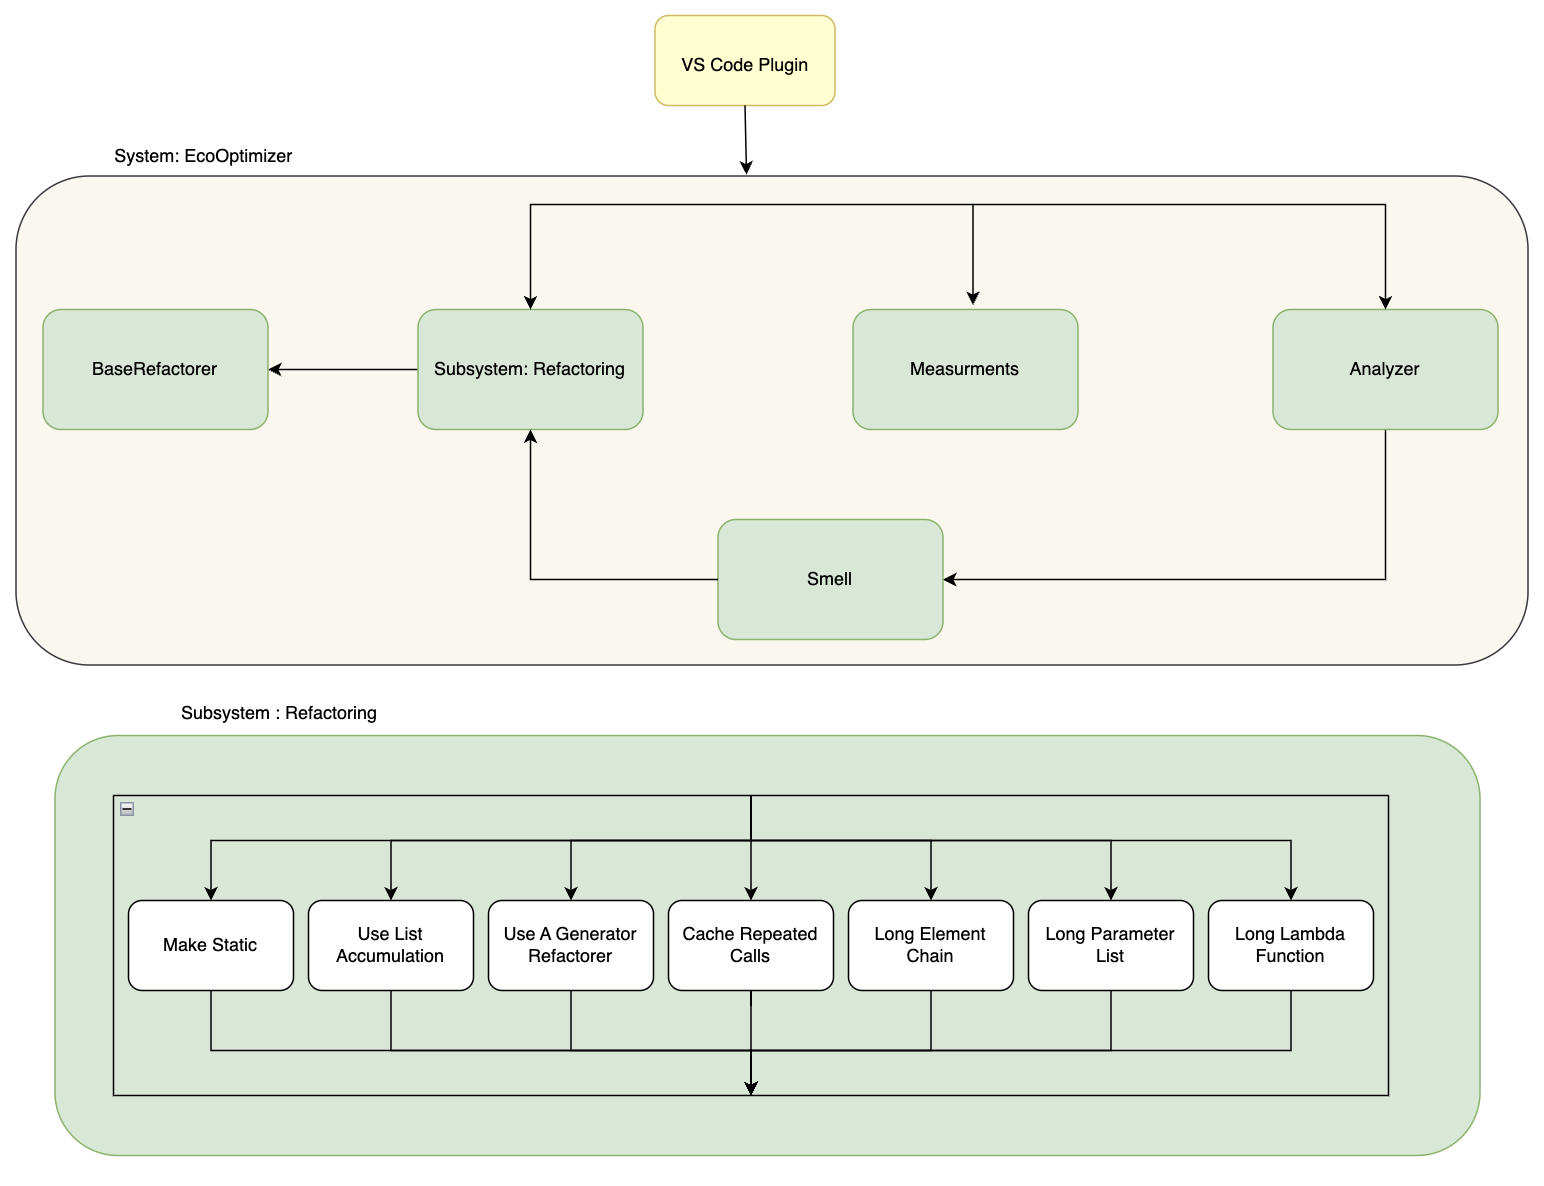
\includegraphics[width=\textwidth]{../../Images/sco_use_diagram.png}
\caption{Use hierarchy among modules}
\label{FigUH}
\end{figure}

\begin{figure}[H]
  \centering
  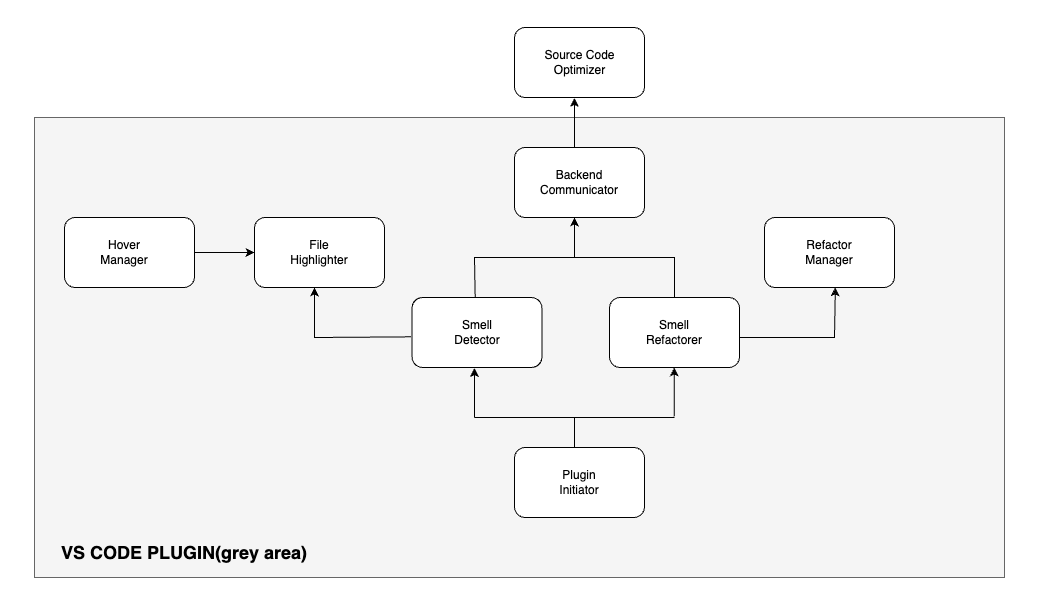
\includegraphics[width=\textwidth]{../../Images/plugin_use_diagram.png}
  \caption{Use hierarchy among modules}
  \label{FigUH_Plugin}
  \end{figure}

%\section*{References} 

\section{User Interfaces}

The project is exposed to the user through the VS Code Plugin, which can be installed 
in any developer's local VS Code Editor. Figure \ref{fig3} highlights the intial interface that 
the user accesses when installating and enabling the plugin. Commands of the plugin are 
available through various routes, one of them is the Command Palette as show in figure \ref{fig4}.

Commands are searchable and can be applied. Figure \ref{fig5} showcases the application of the 
"Eco: Refactor Plugin: Detect Smells" command, which at the end highlights all lines containing 
code smells with yellow lines. On hover, information is available about the specific code smell.
The user also has the option to select or place their cursor on a specific line that they want 
to refactor, and run the "Eco: Refactor Plugin: Refactor Smell" command in order to refactor that 
specific line of code. Figure \ref{fig6} provides a visual of this command in progress, with updates
being provided in bottom right corner.

\begin{figure}[H]
  \centering
  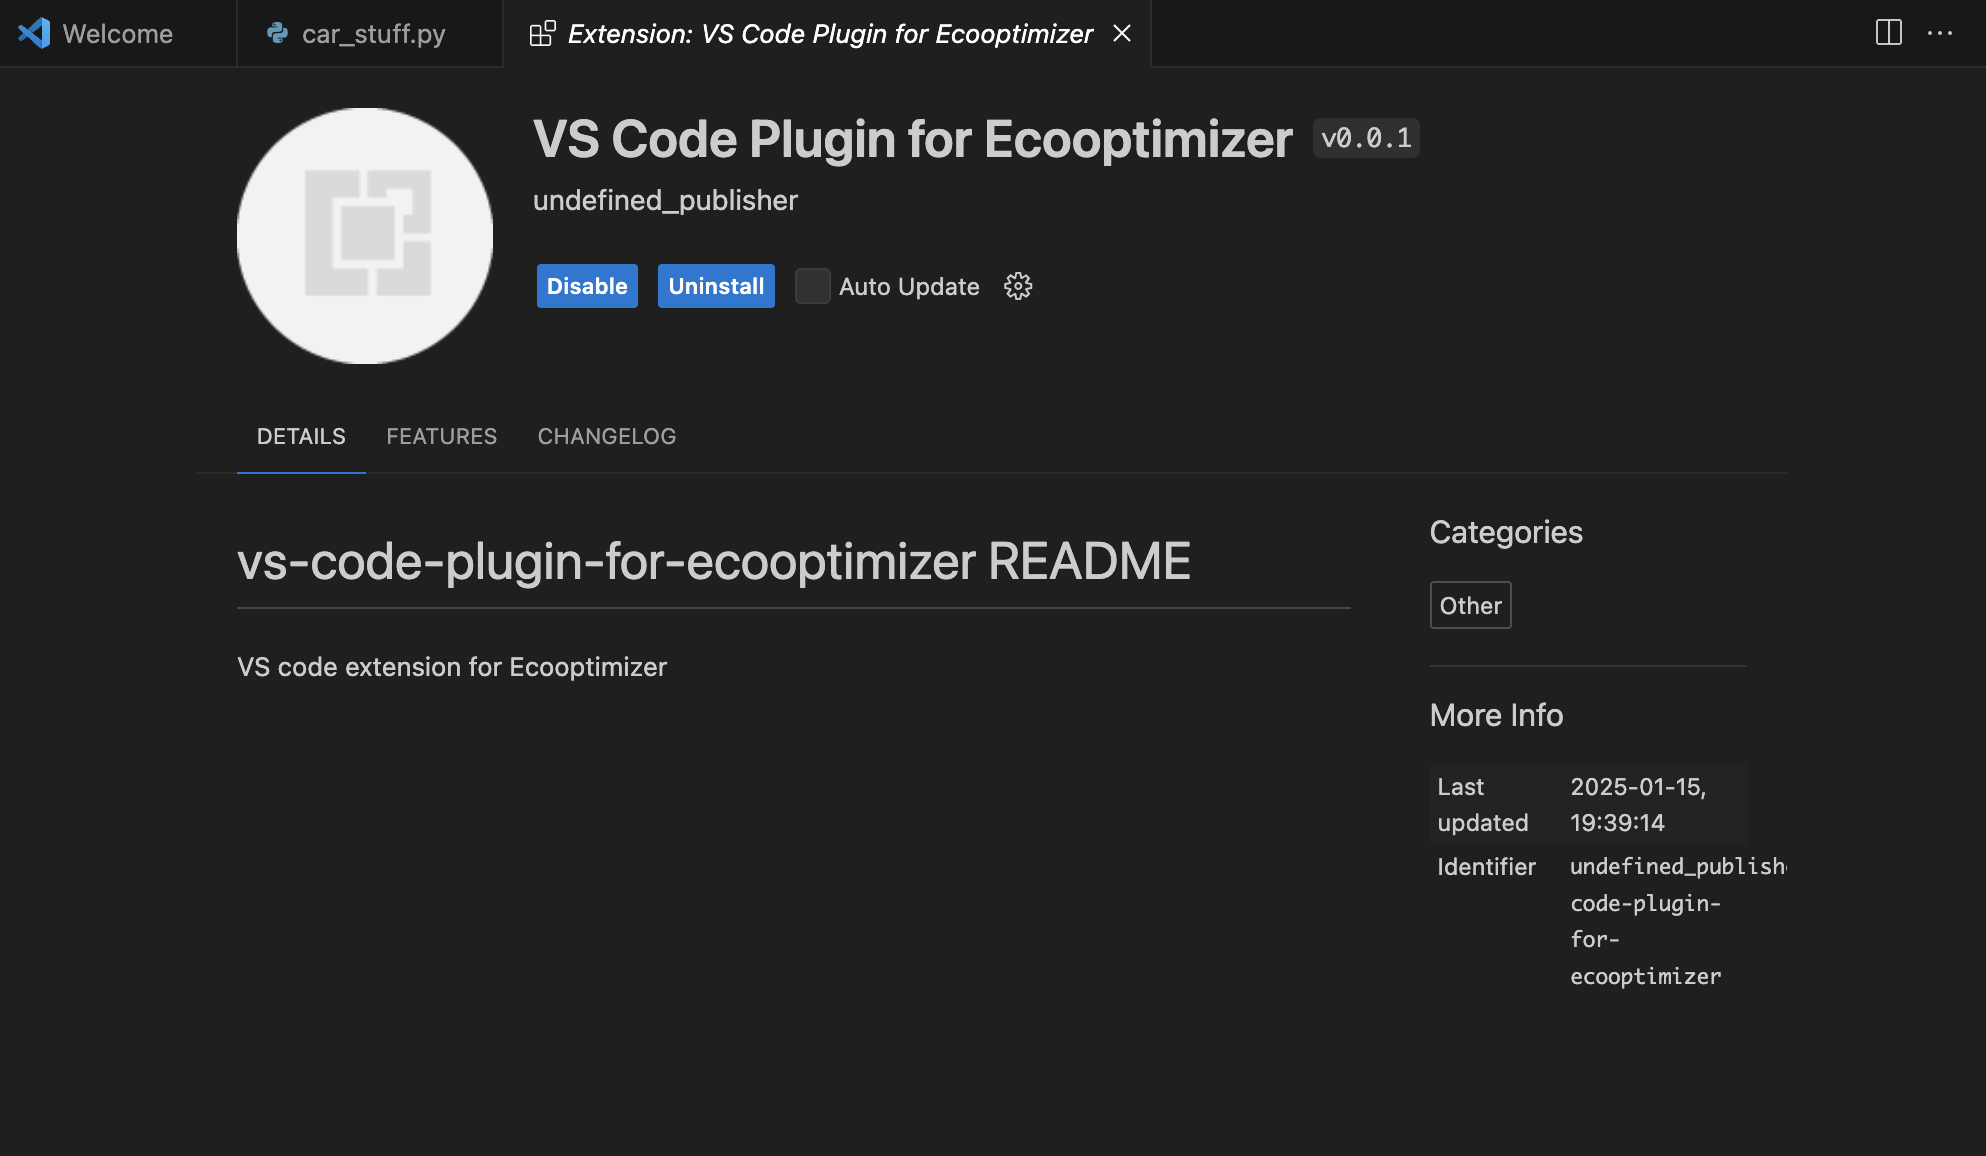
\includegraphics[width=\textwidth]{../../Images/VSPlugin.png}
  \caption{VS Code Plugin Setup}
  \label{fig3}
  \end{figure}
  
  \begin{figure}[H]
  \centering
  
\includegraphics[width=\textwidth]{../../Images/VSPluginCommands.png}
  \caption{VS Code Plugin Commands}
  \label{fig4}
  \end{figure}
  
  \begin{figure}[H]
  \centering
  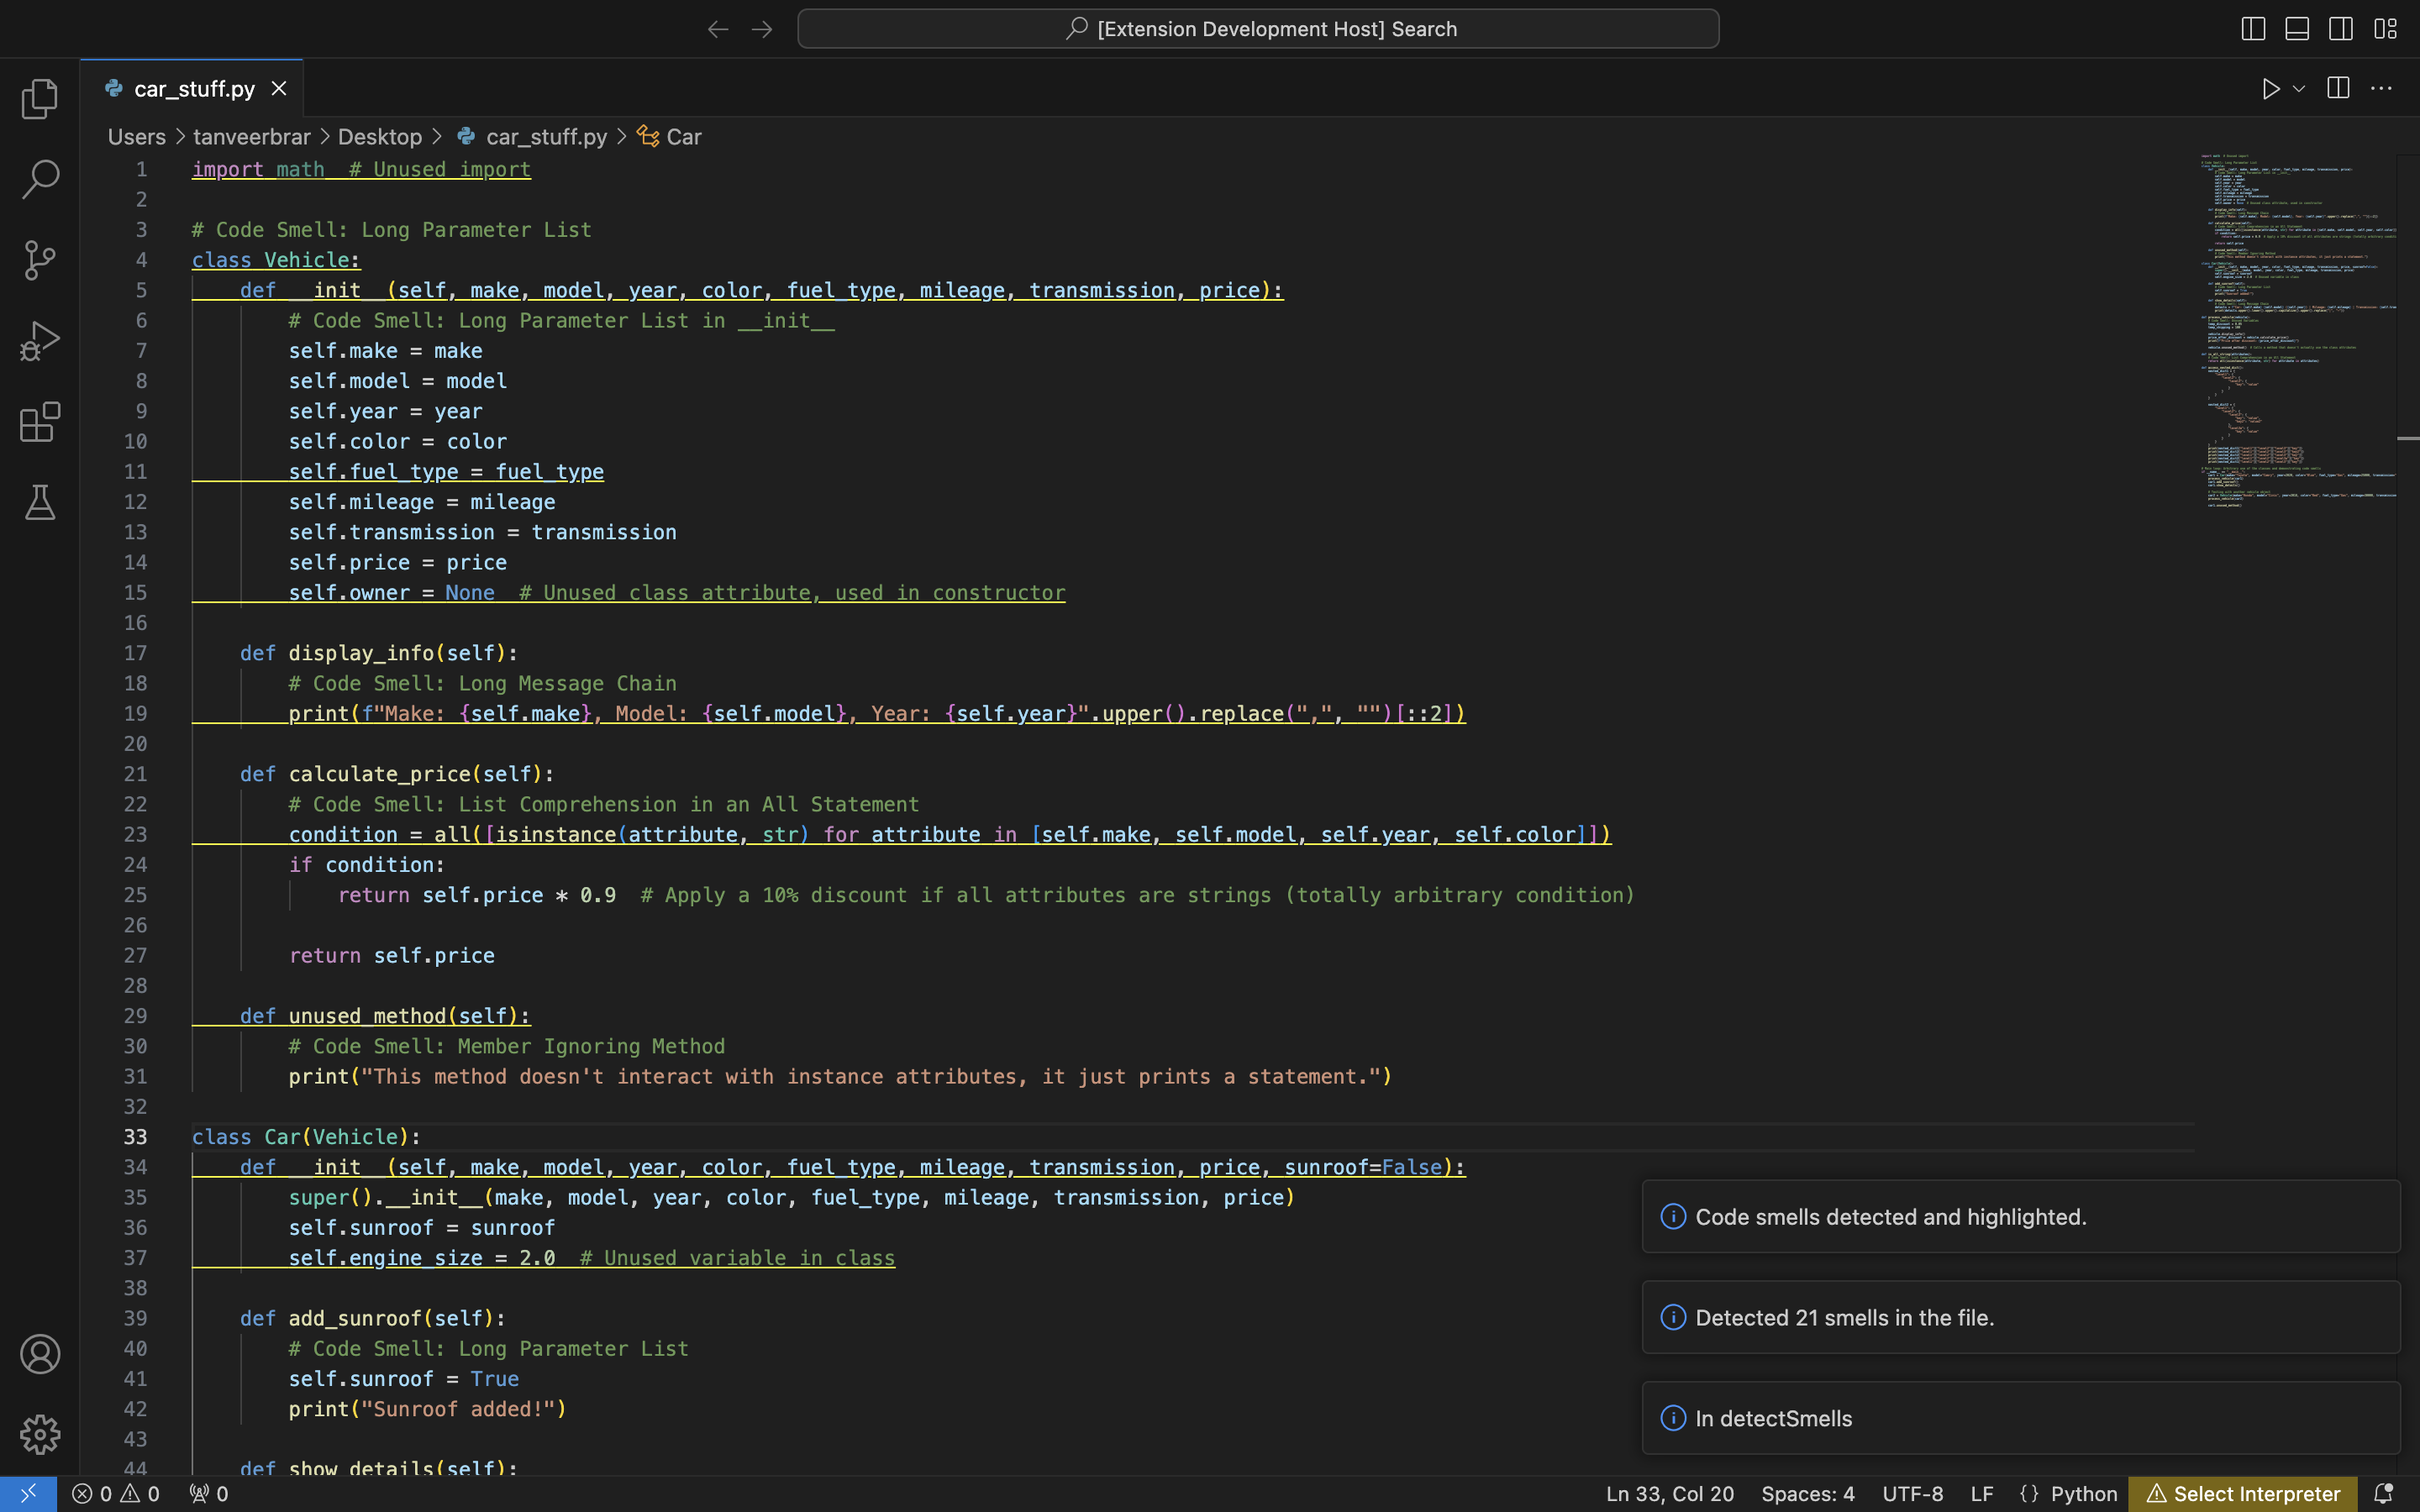
\includegraphics[width=0.7\textwidth]{../../Images/VSPluginDetectMode.png}
  \caption{VS Code Code Analysis Interaction}
  \label{fig5}
  \end{figure}
  
  \begin{figure}[H]
  \centering
  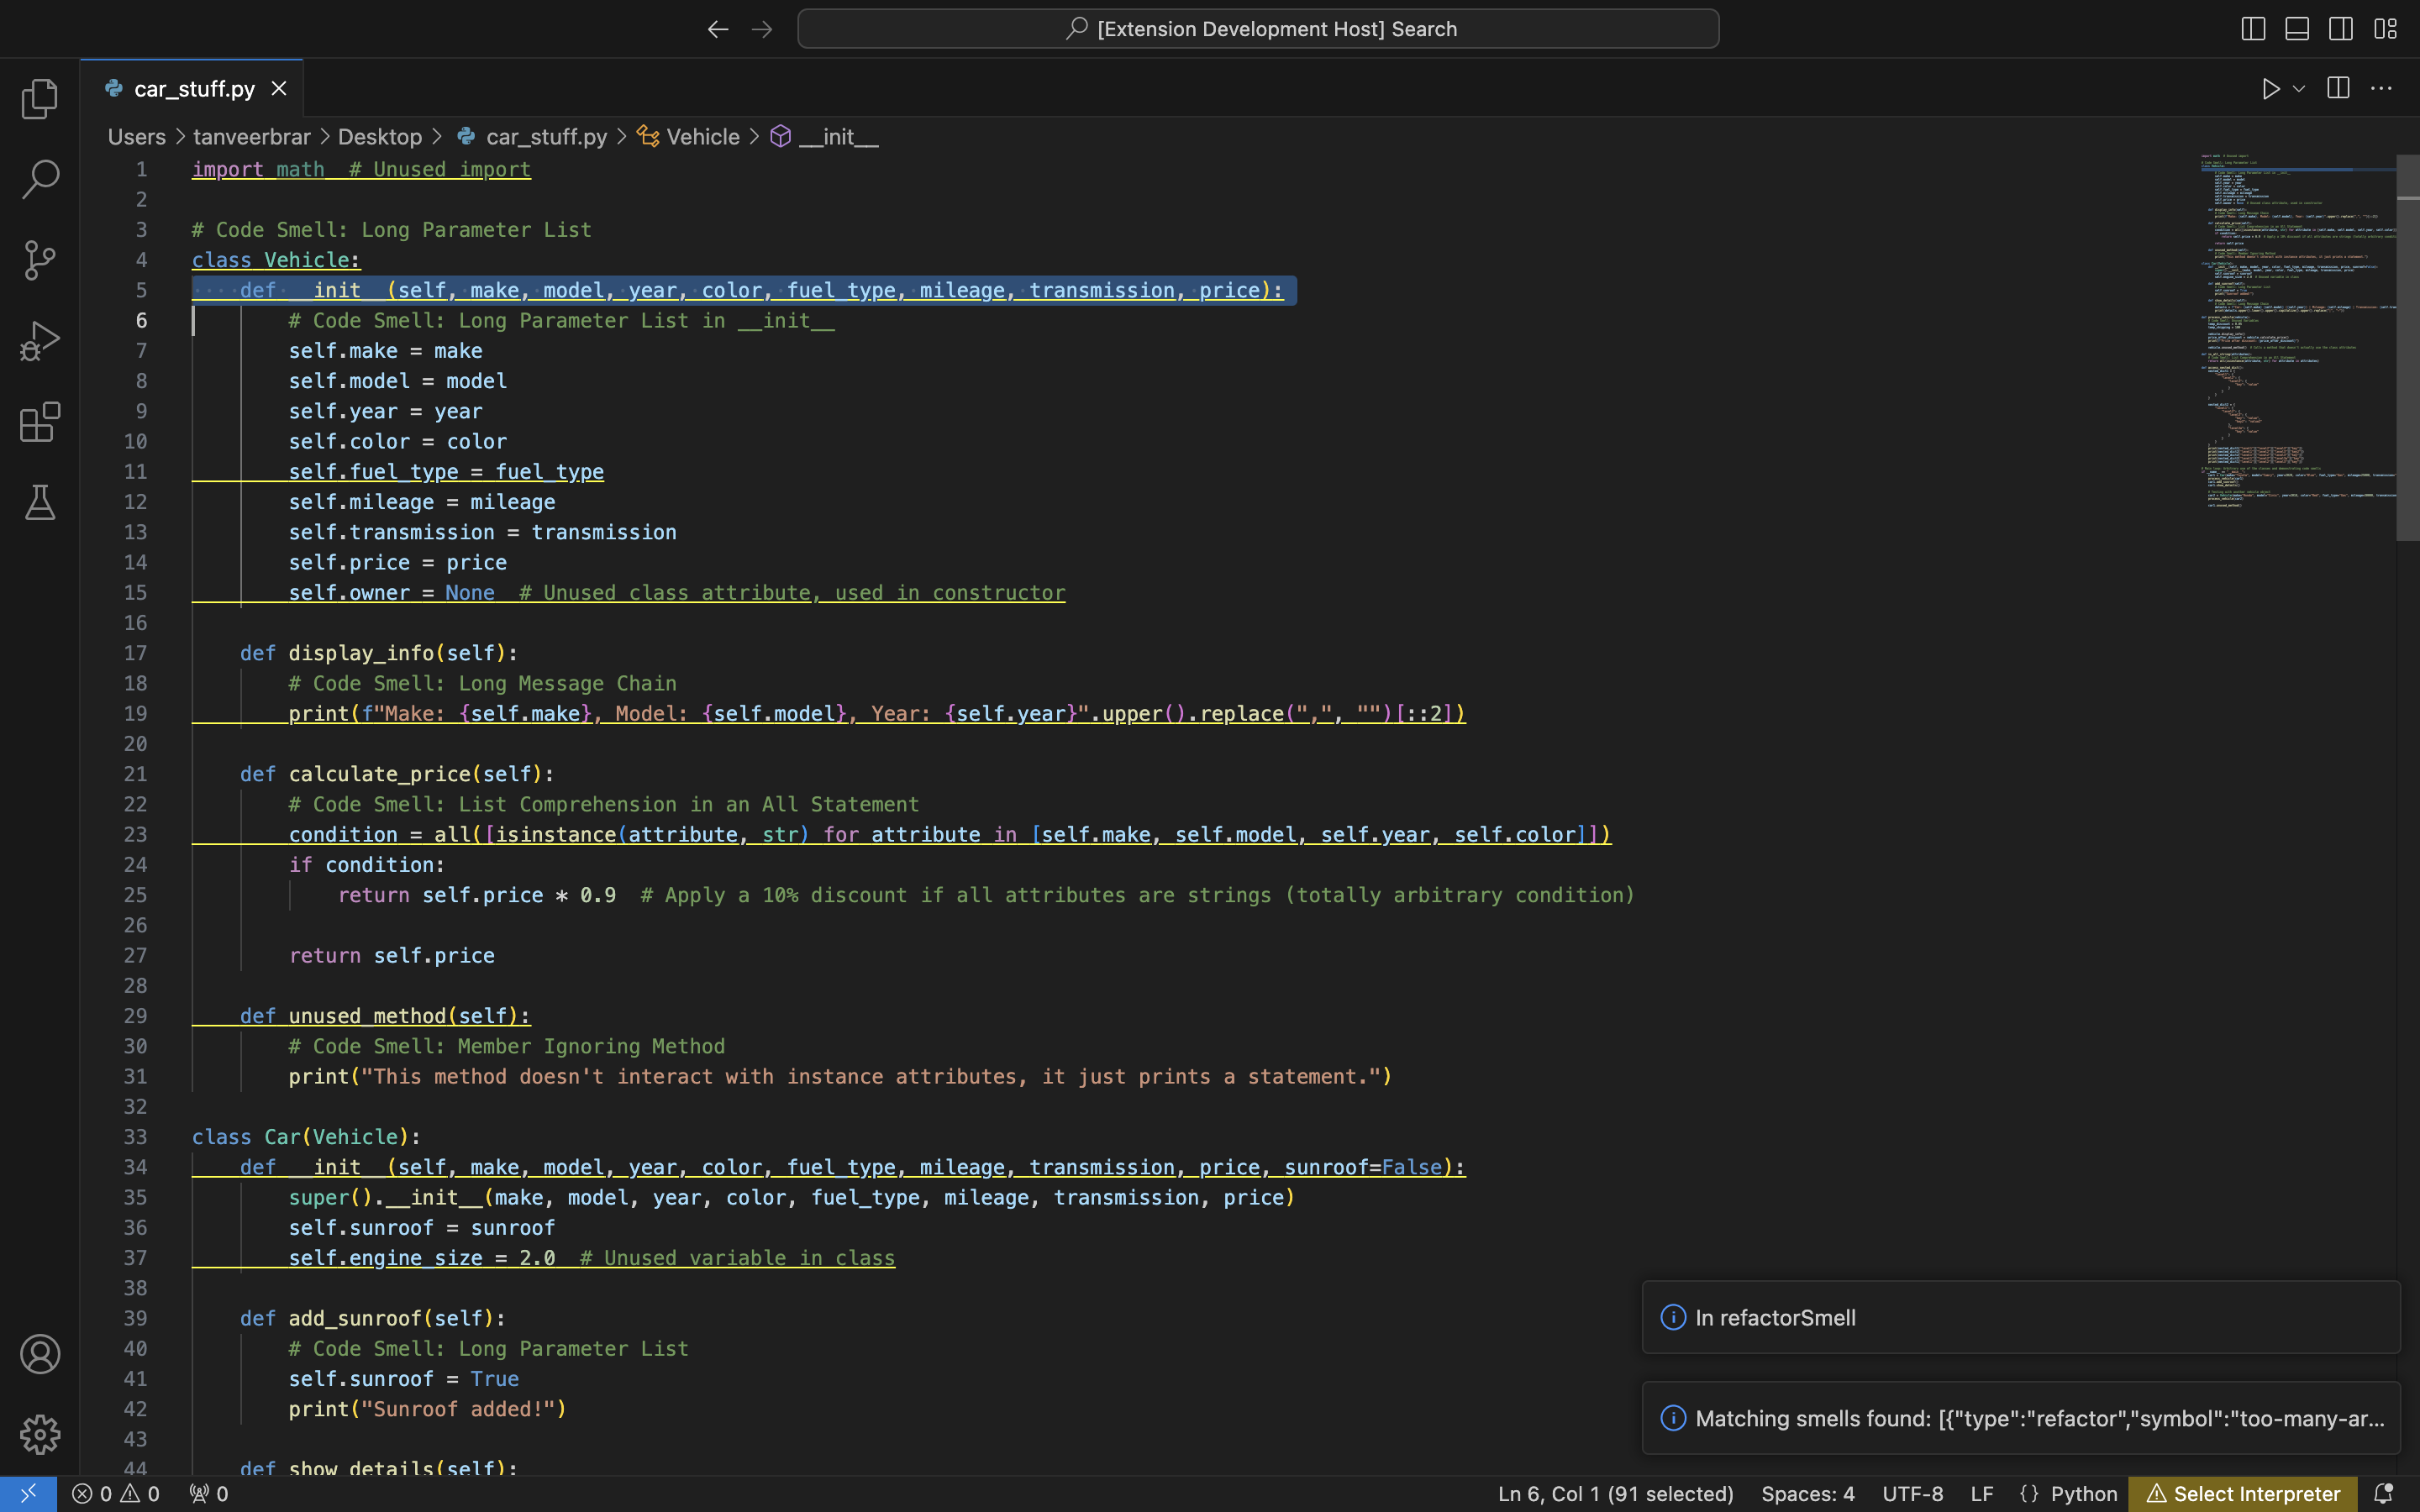
\includegraphics[width=0.7\textwidth]{../../Images/VSPluginRefactorMode.png}
  \caption{VS Code Code Refactoring Interaction(in progress for selected line)}
  \label{fig6}
  \end{figure}


\wss{Design of user interface for software and hardware.  Attach an appendix if
needed. Drawings, Sketches, Figma}

\section{Design of Communication Protocols}

\wss{If appropriate}

\section{Timeline}

All code and corresponding documentation was aimed to be completed before Jan 6th our Demo date for our supervisor.

\begin{table}[h!]
  \centering
  \caption{Timeline}
  \begin{tabular}{|l|l|l|}
  \hline
  \textbf{Module Name} & \textbf{Team Member}        & \textbf{Due Date} \\ \hline
  Base Refactorer                     & Sevhena Walker              & Jan 6, 2025    \\ \hline
  Complex List Comprehension          & Nivetha Kuruparan              & Jan 6, 2025    \\ \hline
  Long Element Chain                  & Ayushi Amin              & Jan 6, 2025     \\ \hline
  Long Lambda Function                & Mya Hussain              & Jan 6, 2025     \\ \hline
  Long Message Chain                  & Mya Hussain              & Jan 6, 2025     \\ \hline
  Member Ignoring Method              & Sevhena Walker             & Jan 6, 2025     \\ \hline
  Repeated Calls                      & Nivetha Kuruparan               & Jan 6, 2025     \\ \hline
  String Concatenation in Loop        & Sevhena Walker              & Jan 6, 2025     \\ \hline
  Long Parameter List                 & Tanveer Brar              & Jan 6, 2025     \\ \hline
  Smell                               & All             & Jan 31, 2025    \\ \hline
  Analyzers                           & All            & Jan 31, 2025      \\ \hline
  Measurements                        & All          & Jan 31, 2025      \\ \hline
  \end{tabular}
  \end{table}
  

\bibliographystyle {plainnat}
\bibliography{../../../refs/References}

\newpage{}

\end{document}